%! TEX root = thesis.tex

\chapter{Introduction}

This thesis is a potpourri of some results that span everything from classical mechanics, to statistical mechanics, to quantum mechanics, to engineering.
A common thread that connects these fields is that of asymptotics and geometry.

\begin{figure}
  \begin{center}
    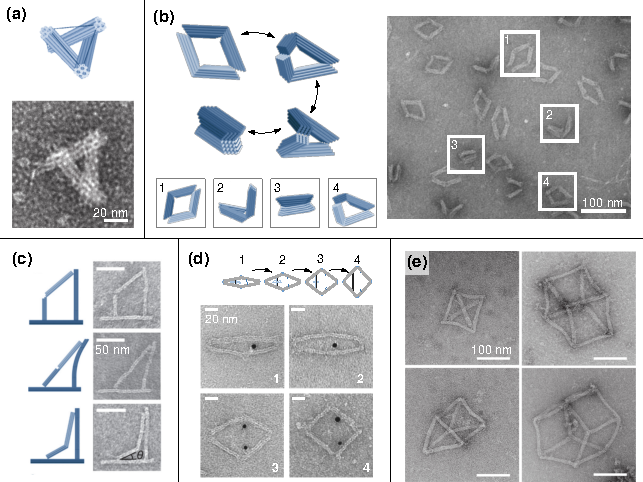
\includegraphics[scale=1.0]{dna.pdf}
  \end{center}
  \caption{DNA origami has been widely used to self assemble a variety of objects at the nanoscale.
    Depicted in the figure are (a) tensegrity structures \cite{liedl2010}; (b), (c) linkage-based mechanisms \cite{marras2015,zhou2015}; (d) a rhombus-shaped nanoactuator~\cite{ke2016}; and (e) self-assembled polyhedra~\cite{iinuma2014}.  All images used with permission.}
  \label{fig:}
\end{figure}

\begin{figure}
  \begin{center}
    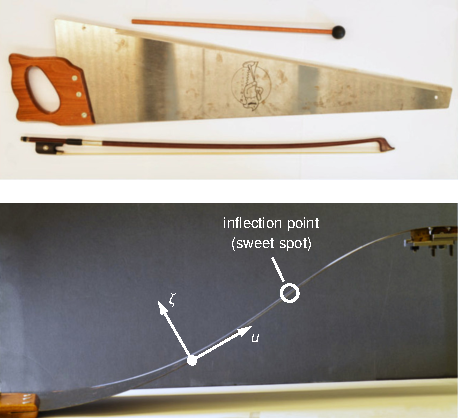
\includegraphics[scale=1.0]{saw/saw.pdf}
  \end{center}
  \caption{%
    An ordinary wood saw when bent into the shape of an S can be played like a musical instrument using a violin bow or a mallet.
    A sustained note is produced on bowing or hitting the saw at its inflection point, which is called a sweet spot by musicians.
    Photographs adapted from Ref.~\cite{shankar2022} and used with permission.
  }
  \label{fig:saw}
\end{figure}


\section{Rigidity theory}

See the notes by \citet{connelly2015} for an introduction to tensegrity structures and the primer by \citet{williams2003} for a slightly advanced treatment.

Forces involved in a state of self stress obey the strong form of Newton's third law and thus cannot possibly result in an unbalanced torque \cite[\S 1.2]{goldstein2002}.
Thus, a tensegrity under self stress is in a state of mechanical equilibrium.
The equilibrium may or may not be stable: again, think of the example with a particle tethered to two walls using springs that are under compression (unstable) or under elongation (stable).

Note that SS exists outside of tensegrity structures.
The only requirement is that all particles interact via central forces.
E.g., one can think of electrostatic analogies, or sticky colloidal clusters.

SS is caused due to linear dependence of constraints.
They might be independent nonlinearly, but on a linear level they are dependent.
Linear constraints are, simply put, hyperplanes.

Maxwell--Calladine theorem is a finite-dimensional toy ``index'' theorem~\cite[\S 2.2]{nakahara2003}.

\subsection{Non-Euclidean origami}

It's easy to understand the configuration manifold of non-Euclidean origami studied by \cite{berry2020}.
A non-Euclidean origami in its ``unfolded'' (or rather, its unactuated) state is not flat.
This means that the linkages forming the origami ``skeleton'' cannot possibly support a self stress since there would be a net unbalanced force in the vertical direction.
Since there can't be a self stress, the Jacobian of the constraint map is full rank everywhere, and thus, the configuration manifold is a smooth 2-dimensional submanifold of $\mathbb{R}^9$ ($M = 7$ and $N = 9$, giving $M - N = 2$).
However, in general, this manifold could be a single connected 2-dimensional manifold or multiple disjoint 2-dimensional manifolds.
If there is positive Gaussian curvature (i.e., an angle deficit) at the center vertex, then the entire structure becomes metastable due to popping up/down of the central vertex.
This popping up and down process is discontinuous and breaks the constraints since the origami has to go through the flat state.
This must be equivalent to having (at least) two 2-dimensional disconnected submanifolds as the configuration space.
When the central vertex has negative Gaussian curvature (i.e., an angle excess), then the origami lacks is metastability.
This must be equivalent to having a single 2-dimensional submanifold as the configuration space.
Note that the manifold can still be disconnected in general, but for the case presenented in \cite{berry2020} it isn't.
What I'm saying is, here there is no reason for the manifold to be connected, but in the previous case (positive Gaussian curvature), it is always disconnected because of physical reasons.
It isn't topology that tells us if the manifolds are disconnected, it's physics.
When there is no Gaussian curvature at the center vertex, the ``unfolded'' state is flat and the origami supports a self stress and the Jacobian drops rank.
This leads to a singularity in the configuration manifold.

\begin{figure}
  \begin{center}
    \includegraphics{zerodof.pdf}
  \end{center}
\caption{A zero \ac{dof} linkage without self stress.  Note how the two constraint manifolds $\mathcal{M}_1$ and $\mathcal{M}_2$ are transverse to each other.}
  \label{fig:hello}
\end{figure}

See the thesis \cite{lengyel2002}.

\begin{figure}
  \begin{center}
    \includegraphics{zerodof_spring.pdf}
  \end{center}
\caption[foo]{A zero \ac{dof} linkage without self stress.  Note how the two constraint manifolds $\mathcal{M}_1$ and $\mathcal{M}_2$ are transverse to each other.}
  \label{fig:hello2}
\end{figure}
\pagebreak

Shape coordinate on a curve can be arclength.  But it's a useless one since it can't be measured experimentally.

Shape space of a triangle is a cone in $\mathbb{R}^{3}$? Joseph Avron's talk at KITP.

Foliation intuitively means that there is a unique hypersurface that passes through each point.

